\documentclass[runningheads]{llncs}\usepackage[]{graphicx}\usepackage[]{color}
%% maxwidth is the original width if it is less than linewidth
%% otherwise use linewidth (to make sure the graphics do not exceed the margin)
\makeatletter
\def\maxwidth{ %
  \ifdim\Gin@nat@width>\linewidth
    \linewidth
  \else
    \Gin@nat@width
  \fi
}
\makeatother

\definecolor{fgcolor}{rgb}{0.345, 0.345, 0.345}
\newcommand{\hlnum}[1]{\textcolor[rgb]{0.686,0.059,0.569}{#1}}%
\newcommand{\hlstr}[1]{\textcolor[rgb]{0.192,0.494,0.8}{#1}}%
\newcommand{\hlcom}[1]{\textcolor[rgb]{0.678,0.584,0.686}{\textit{#1}}}%
\newcommand{\hlopt}[1]{\textcolor[rgb]{0,0,0}{#1}}%
\newcommand{\hlstd}[1]{\textcolor[rgb]{0.345,0.345,0.345}{#1}}%
\newcommand{\hlkwa}[1]{\textcolor[rgb]{0.161,0.373,0.58}{\textbf{#1}}}%
\newcommand{\hlkwb}[1]{\textcolor[rgb]{0.69,0.353,0.396}{#1}}%
\newcommand{\hlkwc}[1]{\textcolor[rgb]{0.333,0.667,0.333}{#1}}%
\newcommand{\hlkwd}[1]{\textcolor[rgb]{0.737,0.353,0.396}{\textbf{#1}}}%
\let\hlipl\hlkwb

\usepackage{framed}
\makeatletter
\newenvironment{kframe}{%
 \def\at@end@of@kframe{}%
 \ifinner\ifhmode%
  \def\at@end@of@kframe{\end{minipage}}%
  \begin{minipage}{\columnwidth}%
 \fi\fi%
 \def\FrameCommand##1{\hskip\@totalleftmargin \hskip-\fboxsep
 \colorbox{shadecolor}{##1}\hskip-\fboxsep
     % There is no \\@totalrightmargin, so:
     \hskip-\linewidth \hskip-\@totalleftmargin \hskip\columnwidth}%
 \MakeFramed {\advance\hsize-\width
   \@totalleftmargin\z@ \linewidth\hsize
   \@setminipage}}%
 {\par\unskip\endMakeFramed%
 \at@end@of@kframe}
\makeatother

\definecolor{shadecolor}{rgb}{.97, .97, .97}
\definecolor{messagecolor}{rgb}{0, 0, 0}
\definecolor{warningcolor}{rgb}{1, 0, 1}
\definecolor{errorcolor}{rgb}{1, 0, 0}
\newenvironment{knitrout}{}{} % an empty environment to be redefined in TeX

\usepackage{alltt}

\usepackage{booktabs} % For formal tables
\usepackage{tikz}
\usepackage{pgfbaselayers}
\usepackage{wrapfig}
\usepackage{multicol}
\usepackage{float}
\usepackage[underline=false]{pgf-umlsd}
\usetikzlibrary{shadows}
\usetikzlibrary{arrows}
\IfFileExists{upquote.sty}{\usepackage{upquote}}{}
\begin{document}



\title{Scaling in concurrent evolutionary algorithms}
% \thanks{Supported by organization x.}}

\titlerunning{Concurrency in evolutionary algorithms}

 \author{Juan J. Merelo\inst{1}
 \and
 J.L.J. Laredo\inst{2}
 \and
 Pedro A. Castillo\inst{1}
 \and
 Jos\'e-Mario Garc\'ia-Valdez\inst{3}
\and
Sergio Rojas-Galeano\inst{4}
}

 \institute{%
   Universidad de Granada/CITIC\\
   Granada, Spain\\
   \email{\{jmerelo,pacv\}@ugr.es}\\
 \and
	RI2C-LITIS, Universit\'e du Havre Normandie\\
   Le Havre, France\\
   \email{juanlu.jimenez@univ-lehavre.fr}\\
 \and
 Instituto Tecnol\'ogico de Tijuana\\
 Calzada Tecnol\'ogico, s/n\\
 Tijuana, Mexico\\
 \email{mario@tectijuana.edu.mx}
 \and
 School of Engineering\\
 Universidad Distrital Francisco Jos\'e de Caldas\\
 Bogot\'a, Colombia\\
 \email{srojas@udistrital.edu.co}
}

\authorrunning{Merelo, J.J. \emph{et al.}}

\maketitle

\begin{abstract}
The concept of \emph{channel}, a computational mechanism
used to convey state to different threads of process execution,
is at the core of the design of multi-threaded concurrent
algorithms. In the case of concurrent evolutionary
algorithms, \emph{channels} can be used to communicate messages 
between several threads performing different evolution tasks 
related to genetic operations or mixing of
populations. In this paper we study to what extent the
design of these messages in a communicating sequential process
context may influence scaling and performance of concurrent
evolutionary algorithms. For this aim, we designed a channel-based
concurrent evolutionary algorithm that is able to effectively solve
different benchmark binary problems (e.g. OneMax, LeadingOnes,
RoyalRoad), showing that it provides a good basis to leverage the
multi-threaded and multi-core capabilities of modern
computers. Although our results indicate that concurrency is
advantageous to scale-up the performance of evolutionary algorithms,
they also highlight how the trade--off between concurrency,
communication and evolutionary parameters affect the outcome of the
evolved solutions, opening-up new opportunities for algorithm design. 
\end{abstract}

\keywords{Concurrency, concurrent evolutionary algorithms, performance
evaluation, algorithm design, distributed evolutionary algorithm}

\section{Introduction}

Despite the emphasis on leveraging newer hardware features
with best-suited software techniques,
 there are not many papers \cite{Xia2010} dealing with the 
creation of concurrent evolutionary algorithms that work in a single
computing node or that extend seamlessly from single to many
computers. In that sense, concurrent programming seems to be the best 
option if we are dealing with a multi-core multi-threaded processor architecture 
where many processes and threads can coexists at the same time. The latter 
implies applications (and algorithms) should be able to leverage those
processes to take full advantage of their capabilities.

The best way to do so is
to match those capabilities at an abstract level by languages
that build on them so that high-level algorithms can be implemented without
worrying about the low-level mechanisms of creation or destruction of
threads, or how data is shared or communicated among them. These
languages are called concurrent, and the programming paradigm
implemented in them concurrency-oriented programming or simply
concurrent programming \cite{Armstrong2003}.

These languages, that include Perl 6, Go, Scala and Julia, usually support 
programming constructs that manage threads like first class
objects, including operators for acting upon them and to using them as 
function's input or return parameters. The latter have implications in 
the coding of concurrent algorithms due to the
direct mapping between patterns of communication and processes with
% patterns of communication between processes? - Mario 
% no, two different things  - JJ
language expressions: on the one hand it simplifies coding because higher-level
abstractions for communication are available; on the other hand
it changes the paradigm for implementing algorithms, since these new
communication constructs and the overhead they bring to processing
data need to be considered.

Moreover, concurrent programming adds a layer of abstraction over the parallel
facilities of processors and operating systems, offering a
high-level interface that allows the user to program modules of code to
be executed in parallel threads \cite{andrews1991concurrent}.

Different languages offer different concurrency strategies depending
on how they deal with shared state, 
that is, data structures that could be accessed from several processes or
threads. In this regard, there are two major fields and other, less well known models using, for instance, tuple
  spaces \cite{gelernter1985generative}:
\begin{itemize}
\item Actor-based concurrency \cite{schippers2009towards}
totally eliminates shared state by introducing a series of data
structures called {\em actors} that
store state and can mutate it locally. 
\item Process calculi or process algebra is a framework to describe
  systems that work with independent
  processes interacting between them using channels. One of the best
  known is called the {\em communicating sequential processes} (CSP)
methodology \cite{Hoare:1978:CSP:359576.359585}, which is effectively
stateless, with different processes reacting to a channel input without
changing state, and writing to these channels. Unlike actor based
concurrency, which keeps state local, in this case per-process state is totally
eliminated, with all computation state managed as messages in a channel.
\end{itemize}

Many modern languages, however, follow the CSP abstraction, and it has
become popular since it fits well other programming paradigms, like
reactive and functional programming, and allows for a more efficient
implementation, with less overhead, and with well-defined
primitives. This is why we will use it in this paper for creating  {\em natively}
concurrent evolutionary algorithms. We have chosen Perl 6, although 
other alternatives such as Go and Julia are feasible.

In previous papers
%\cite{Merelo:2018:MEA:3205651.3208317:anon,merelo:WEA:anon}
\cite{Merelo:2018:MEA:3205651.3208317,merelo:WEA} we
designed an evolutionary algorithm that fits well this architecture
and explored its possibilities. That initial exploration showed that
a critical factor within this algorithmic model is the communication
between threads; therefore designing
efficient messages is high-priority to obtain good algorithmic
performance and scaling. In this paper, we will test several
communication strategies: a loss-less one that compresses the population,
and a lossy one that sends a representation of gene-wise
statistics of the population.

The rest of the paper is organized as follows: next we present the
state of the art in concurrency in evolutionary algorithms, followed
by Section \ref{sec:design} on the design of concurrent EAs in Perl 6. 
Experimental results are presented next in Section
\ref{sec:exp}; finally, we discuss our conclusions in Section
\ref{sec:conclusions}. 

\section{State of the Art}

% The problem of communication/synchronization
% between processes or threads has been the subject of long-standing study,
% to fully leverage the multiple
% processors and cores on a given machine. 
The parallelization of nature-inspired
optimization algorithms has been an active field, allowing researchers 
to solve complex optimization problems having a high computational 
cost \cite{Lalwani2019}. In the literature, most works are concerned 
with process-based concurrency, using, for instance, a Message Passing Interface 
(MPI) \cite{gropp1999using}, or hybrids with fine-grain
parallelization by using libraries such as OpenMP \cite{dagum1998openmp}
that offer multi-threading capabilities \cite{jin2011high}. Recent trends
in software development have motivated the inclusion of new 
constructs to programming languages to simplify
the development of multi-threaded programs. The theoretical support 
used by these implementations is based on CSP. Languages such as Go 
and Perl 6 implement this concurrency model as an abstraction for 
their multi-threading capabilities. (the latter including additional mechanisms such as 
{\em promises} or low-level access to the creation of threads). Even 
interpreted languages with a global interpreter lock, such as Python also
have included {\em promises} and {\em futures} in their latest versions,
to leverage intensive multi-threading IO capabilities.
% Using these native capabilities give developers the advantage of
% having less error-prone implementations which are more readable, concise, and
% following language conventions. 




% I think there could be confusion between the general "process" part 
% of an algorithm (from Process calculi), and an OS process (an instance of a program).a   
% So there is inter-process comunication/synchronization and
% inter-thread comunication/synchronization. For instance, Python can
% do a real parallel execution using processes and they can communicate 
% between them (RPC, RMI, Shared memory, message queues, etc.)
% Here, I think we are dealing only with communication between 
% threads. Python on the other hand cannot use two threads at the
% same time. - Mario


%One of the 
%best efforts to formalize and simplify that matter 
%is Hoare's {\em Communicating Sequential Processes} \cite{Hoare:1978:CSP:359576.359585},
%that proposes an interaction description language which is the 
%theoretical support for many libraries and modern programming 
%languages. In such model, concurrent programs communicate on 
%the basis of {\em channels}, a sort of pipe buffer used to
%interchange messages between the different processes or threads, 
%either asynchronously or synchronously. 

The fact that messages have to be processed without secondary effects
and that actors do not share state makes concurrent
programming specially fit for languages with
functional features; this has made this paradigm specially popular for
late cloud computing implementations; however, its reception 
in the EA community has been scarce \cite{Hawkins:2001:GFG:872017.872197}, 
although some efforts have lately revived
the interest for this paradigm \cite{swan2015research}.
Several years ago it was used in Genetic Programming
\cite{Briggs:2008:FGP:1375341.1375345,Huelsbergen:1996:TSE:1595536.1595579,walsh:1999:AFSFESIHLP}
and recently in neuroevolution \cite{Sher2013} and program synthesis \cite{valkov2018synthesis} 
using the functional programming features of the Erlang language
 for building an evolutionary multi-agent system \cite{barwell2017using}.

% Regarding functional languages, Erlang and Scala have
% embraced the actor model of concurrency and get excellent results in
% many application domains; Clojure is another one with concurrent
% features such as promises/futures, software transactional memory (STM) 
% and agents; Kotlin \cite{simson2017open} has been recently used for
% implementing a functional evolutionary algorithm framework.  
% 
% On the
% other hand, Perl 6 \cite{Tang:2007:PRI:1190216.1190218,lenzperl} 
% uses different concurrency models, varying from implicit concurrency 
% using the {\tt hyper} and {\tt race} functions, that automatically 
% parallelize operations on iterable data structures, to explicit 
% concurrency using threads. 
% The {\tt Algorithm::Evolutionary::Simple} library introduced last year
% %\cite{DBLP:conf/gecco/GuervosV18}
% .

Earlier efforts to study the issues of concurrency in EA are worth 
mentioning. For instance, the EvAg model \cite{evag:gpem} resorts to 
the underlying platform scheduler to manage the different threads of 
execution of the evolving agents; in this way the model scaled-up 
seamlessly to take full advantage of CPU cores. In the same avenue 
of measuring scalability,  experiments were conducted
in \cite{wcci:evoag} comparing single and a dual-core processor 
concurrency achieving near linear speed-ups. The latter
was further on extended in \cite{DBLP:conf/evoW/LaredoBMG12} by scaling
up the experiment to up to 188 parallel machines, reporting speed-ups 
up to $960\times$, nearly four times the expected linear growth 
in the number of machines (when local concurrency were not taken 
into account). Other authors have addressed explicitly multi-core 
architectures, such as Tagawa \cite{Tagawa201212} which used 
shared memory and a clever mechanism to avoid deadlocks. Similarly,
\cite{kerdprasop2012concurrent} used a message-based architecture 
developed in Erlang, separating GA populations as different
processes, although all communication was taking place with a common
central thread. 

In previous papers 
%\cite{Merelo:2018:MEA:3205651.3208317:anon,Garcia-Valdez:2018:MEA:3205651.3205719:anon},
\cite{Merelo:2018:MEA:3205651.3208317,Garcia-Valdez:2018:MEA:3205651.3205719},
we presented a proof of concept of the implementation of a stateless 
evolutionary algorithms using Perl 6, based on a single 
channel model communicating threads for population evolving and 
mixing. In addition, we studied the effect of running parameters 
such as the {\em generation gap} (similar to the concept of {\em
time to migration} in parallel evolutionary algorithms) and 
population size, realizing that the choice of parameters may have 
a strong influence at the algorithmic level, but also at the 
implementation level, in fact affecting the actual wallclock
performance of the EA.

%\section{Setting up the experiments using an evolutionary algorithm library in Perl 6}
\section{Design of a concurrent evolutionary algorithm in Perl6}
\label{sec:design}

Perl 6 is a concurrent, functional language
\cite{DBLP:journals/corr/abs-1809-01427} which was conceived with the
intention of providing a solid conceptual framework for multi-paradigm
computing, including thread-based concurrency and asynchrony. It's got
a heuristic layer that optimizes code during execution time. In the last few
years, performance of programs written in Perl 6 has been sped-up by a 100x factor, 
approaching the same scale of other interpreted
languages, although still with some room for improvement.

The {\tt Algorithm::Evolutionary::Simple} Perl 6 module was published
in the ecosystem a year ago and got recently into version 0.0.7. It
is a straightforward implementation of a canonical evolutionary
algorithm with binary representation and includes building blocks for
a generational genetic algorithm, as well as some fitness functions
used generally as benchmarks.

% Those evolutionary algorithm building blocks do not include concurrent
% primitives; it's up to the developer to design a concurrent
% evolutionary algorithm using it.

The baseline we are building upon, is similar to the one used in previous experiments
%\cite{Merelo:2018:MEA:3205651.3208317:anon}
\cite{Merelo:2018:MEA:3205651.3208317}. Our intention was to
create a system that was not functionally equivalent to a sequential
evolutionary algorithms, that also follows the principle of
CSP. We decided to allow the algorithm to implement several threads communicating state through
channels. Every process itself will be stateless, reacting to the
% Please consider for other papers: Every 'subroutine' itself will be stateless, reacting to the... - Mario
presence of messages in the channels it is listening to and sending
result back to them, without changing state.

As in the previous papers, \cite{merelo:WEA},% \cite{merelo:WEA:anon}, 
we will use two groups of threads and two channels. 
The two groups of threads perform the following functions:\begin{itemize}
\item The {\em evolutionary} threads will be the ones performing 
the operations of the evolutionary algorithm.
\item The {\em mixing} thread will take existing populations, to create
  new ones as a mixture of them.
\end{itemize}

% \begin{figure}[h!tb]
%   \centering
\begin{wrapfigure}[16]{l}{0.35\columnwidth}
  %\centering
  \vspace{-.5\intextsep}
\hspace*{-.8\columnsep}
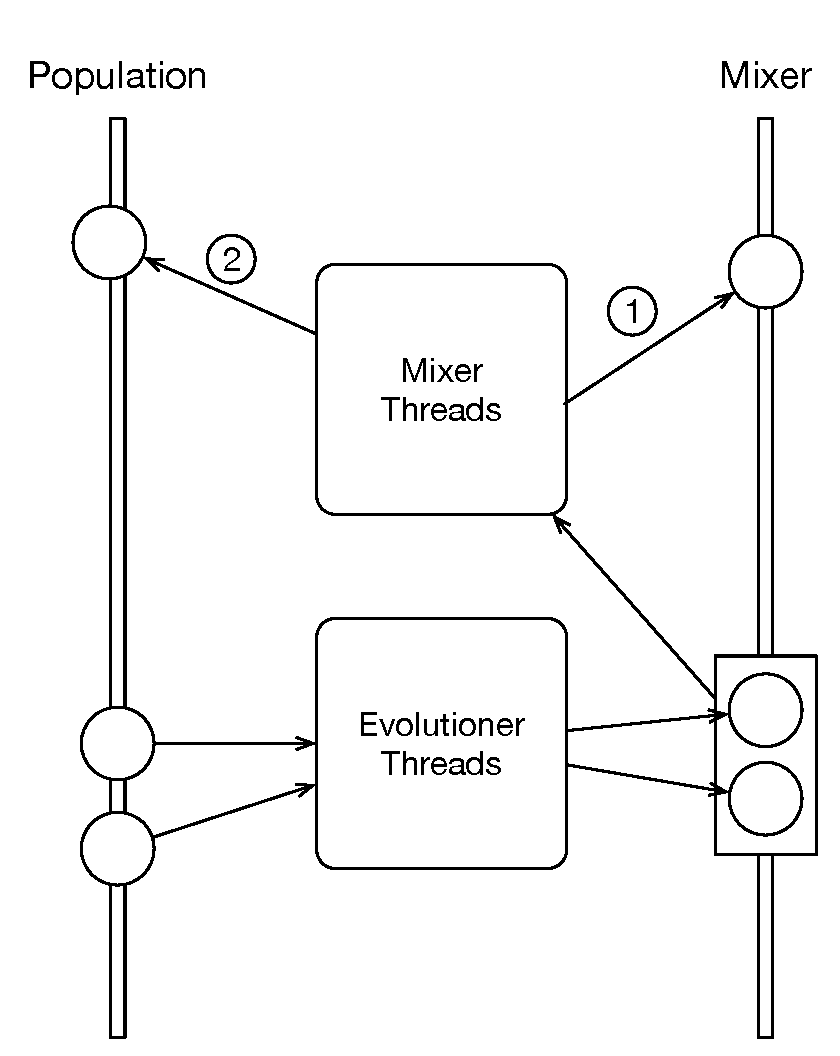
\includegraphics[width=0.35\columnwidth]{../figure/popmixer}
\caption{General scheme of operation of channels and thread groups. }
\label{fig:scheme}
\end{wrapfigure}
% \end{figure}


Besides, the two channels carry messages consisting of populations,
but they do so in a different way:\begin{itemize}
  
\item The {\em evolutionary} channel will be used for carrying
  non-evolved, or generated, populations.
\item The {\em mixer} channel will carry, {\em in pairs}, evolved
  populations. 
\end{itemize}

These will be connected as shown in Figure \ref{fig:scheme}. The
evolutionary thread group will read only from the evolutionary channel,
evolve for a number of generations, and send the result to the mixer
channel; the mixer group of threads will read only from the mixer
channel, in pairs. From every pair, a random element is put back into
the mixer channel, and a new population is generated and sent back to
the evolutionary channel. 

% \begin{figure}[h!tb]
%   \centering
\begin{wrapfigure}[29]{r}{0.55\columnwidth}
  \centering
  \vspace{-.5\intextsep}
\hspace*{-.8\columnsep}
\scalebox{.6}{
\begin{sequencediagram}

\newthread[red]{E}{Evolver} 

\tikzstyle{inststyle}+=[rounded corners=3mm] 
\newinst{C}{Channel}

\tikzstyle{inststyle}+=[rounded corners=0]
\newthread[blue]{M}{Mixer}

\begin{call}{E}{evolve()}{E}{}\end{call}

\setthreadbias{east}
\begin{messcall}{E}{$pop_1$}{C} 
\mess{C}{$pop_1$}{M}
\end{messcall}

\prelevel\prelevel
\begin{call}{E}{evolve()}{E}{}\end{call}

\setthreadbias{east}
\begin{messcall}{E}{$pop_2$}{C}  
\mess{C}{$pop_2$}{M}
\end{messcall}

\prelevel\prelevel
\begin{call}{M}{mix()}{M}{}\end{call}

\postlevel\postlevel
\setthreadbias{west}
\begin{messcall}{M}{\shortstack{ \{\ $mixpop_1$,\\ $mixpop_2$,\\ \vdots \\ $mixpop_k$ \} }}{C}

\mess{C}{$mixpop_1$}{E} 
\begin{call}{E}{evolve()}{E}{}\end{call}

\setthreadbias{east}
\begin{messcall}{E}{$pop_3$}{C} 
\postlevel
\mess{C}{$mixpop_2$}{E} 
%\prelevel
\mess{C}{$pop_3$}{M}
\end{messcall}

\prelevel\prelevel
\begin{call}{E}{evolve()}{E}{}\end{call}

\setthreadbias{east}
\begin{messcall}{E}{$pop_4$}{C}
\mess{C}{$pop_4$}{M}
\end{messcall}

\setthreadbias{west}
\prelevel
\mess{C}{$mixpop_k$}{E}%\end{messcall}

\end{messcall}

\prelevel\prelevel
\begin{call}{M}{mix()}{M}{\vdots}\end{call}
\prelevel
\begin{call}{E}{evolve()}{E}{\vdots}\end{call}

\end{sequencediagram}
}

\caption{Communication between threads and channels for
  concurrent EAs. The two central bars represent the channel, and
  color corresponds to their roles: blue for mixer, red for evolver. 
  Notice how the evolver threads always read from the mixer channel, 
  and always write to the evolver channel.}
\label{fig:schematic}
% \end{figure}
\end{wrapfigure}

The main objective of using two channels is
to avoid deadlocks; the fact that one population is written always
back to the mixer channel avoids starvation of the channel. 
Figure \ref{fig:schematic} illustrates this operation, where the
timeline of the interchange of messages between the evolver and mixer
threads and evolver and mixer channels is clarified.

The state of the algorithm will be transmitted via messages that
contain data about one population. Since using the whole population
will incur in a lot of overhead, we use a strategy that is inspired in {\em EDA}, 
or Estimation of Distribution Algorithm: instead of 
transmitting the entire population, the message sent to the channel 
will consist of a prototype array containing the probability distribution 
across each gene in the population. In this sense,
this strategy is similar to the one presented by de la Ossa et
al. in \cite{10.1007/978-3-540-30217-9_25}. 
  
Nonetheless, our strategy differs from a pure EDA in that once the evolutionary
thread have internally run a canonical genetic algorithm, it takes 
only the top quartile of best individuals to compute an array with the 
probability distribution of their genes (computed with frequentist rules) 
and then compose the message that is sent to the {\em mixer} threads. 
  
A {\em mixer} thread, in turn, 
builds a new prototype array by choosing randomly at each gene location
one probability parameter out of the  two {\em populations} (actually, distributions), 
instead of working directly on individuals. While in the baseline strategy the
selection took place in the mixer thread by eliminating half the
population, in this new design the selection occurs in the evolutionary thread
that selects the 25\% best individuals to compose the probability distribution
message. When the evolver thread reads the message back, it generates a new population 
using the mixed distribution obtained by the mixer.

\section{Experimental results}
\label{sec:exp}

We focused on the scaling capabilities of the algorithm
and implementation, so we tested several benchmark, binary functions:
OneMax, Royal Road and Leading Ones, all of them with 64 bits (for function definitions see e.g. \cite{rojas2012memory}). 

\begin{figure*}[h!tb]
  \centering
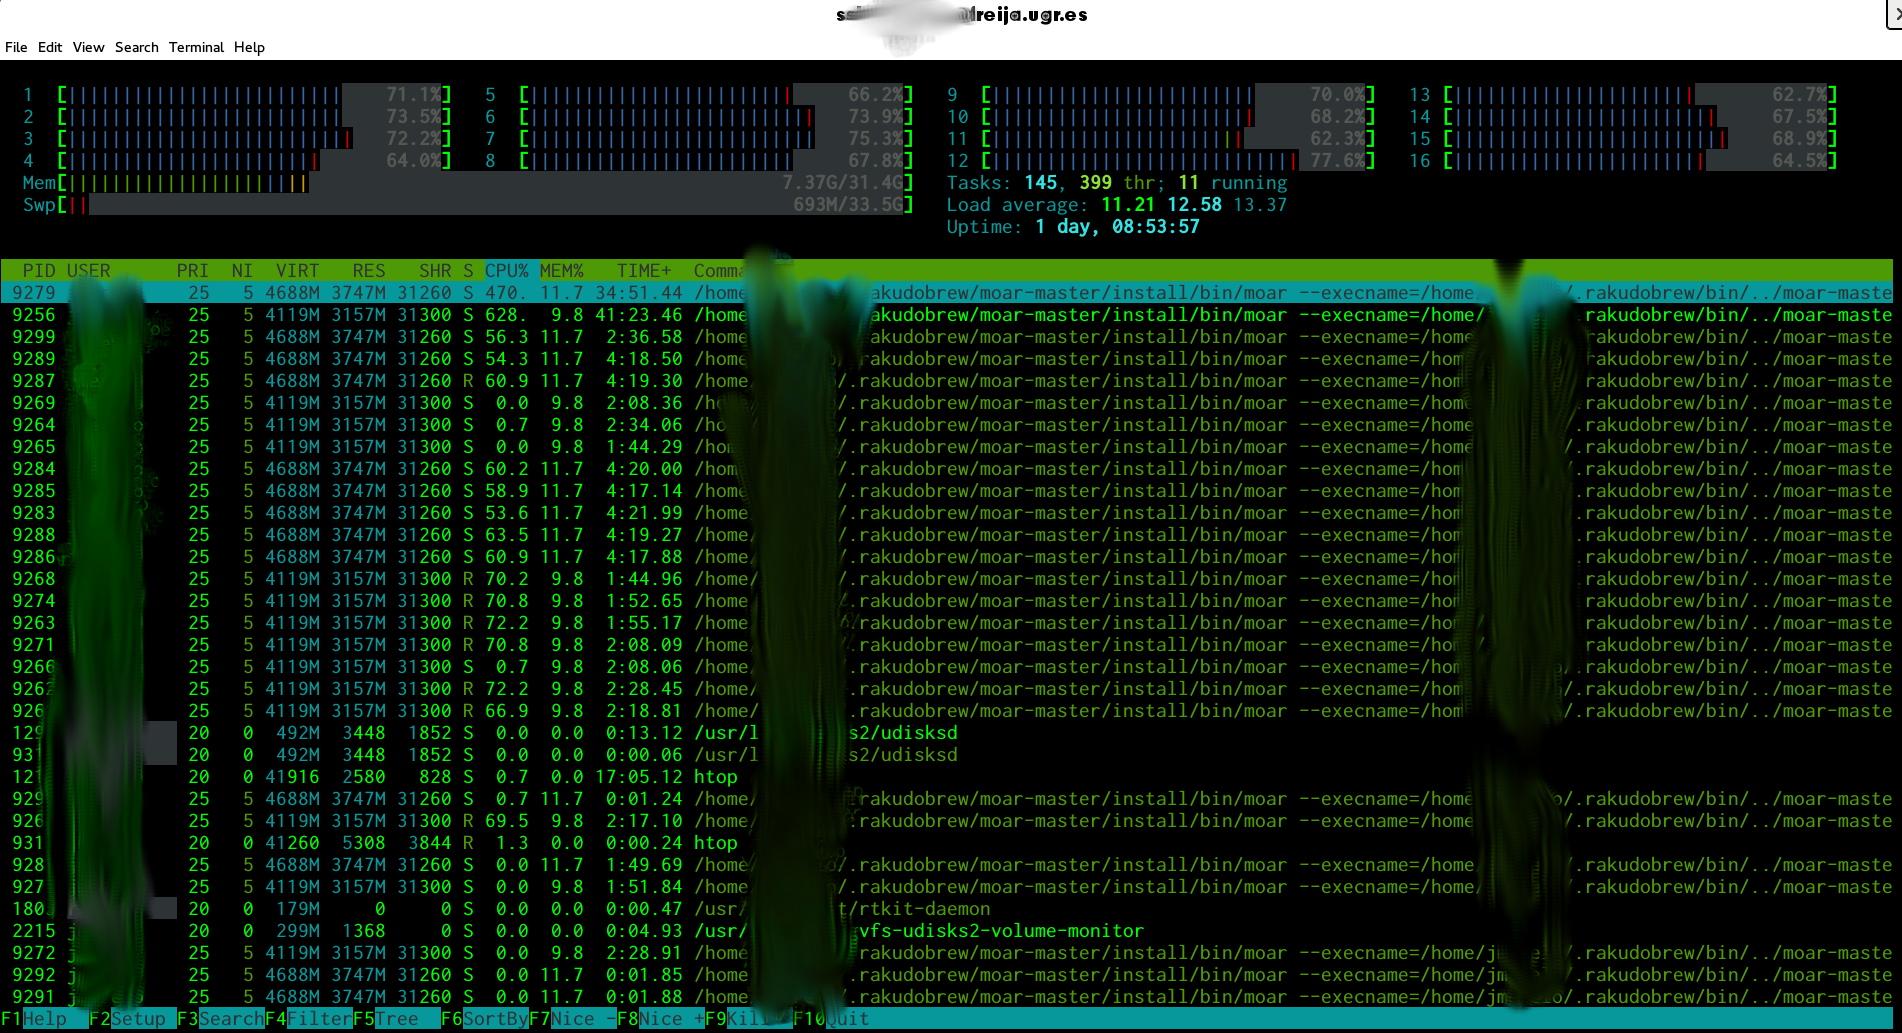
\includegraphics[width=.99\textwidth]{../figure/screenshot}
\caption{An htop utility screenshot for the used machine running
  two experiments simultaneously. It can be seen all processors
  are kept busy, with a very high load average. }
\label{fig:screenshot}
\end{figure*}
%
However, the intention of concurrent evolutionary algorithms is to
leverage the power of all threads and processors in a computer 
so we must find out how it scales for different fitness functions. 
We are setting the number of initial populations to the
number of threads plus one, as the minimum required to avoid
starvation, and we are using a single mixing thread. 
As reported in our previous papers %\cite{Merelo:2018:MEA:3205651.3208317:anon,Garcia-Valdez:2018:MEA:3205651.3205719:anon}, 
\cite{Merelo:2018:MEA:3205651.3208317,Garcia-Valdez:2018:MEA:3205651.3205719},
we are dividing the total population by the number of threads. 
The population size will be 1024 for OneMax, 8192 for Royal Road 
and 4096 Leading Ones. These quantities were found heuristically 
by applying the bisection method on a selectorrecombinative algorithm, 
which doubles the population until one that is able to find 
the solution 95\% of the time is found.

Experiments were run on a machine with the
Ubuntu 18.04 OS and an AMD Ryzen 7 2700X Eight-Core Processor
at 3.7GHz, which theoretically has 8 x 16 = 128 physical
threads. Figure \ref{fig:screenshot} shows the utility  {\tt htop} with an 
experiment running; the top of the screen shows the rate at which all
cores are working, showing all of them occupied; of course, the
program was not running exclusively, but the list of processes below
show how the program is replicated in several processor, thus
leveraging their full power. 

Observe also the number of threads
that are actually running at the same time, 
a few of which are being used by our application; these are not, however, 
physical but operating system threads; 
the OS is able to accommodate many more threads that are physically 
available if the code using them is idle. 

%
We are firstly interested in the number of evaluations needed to find
the solution (see Fig. \ref{fig:threads1}), since as
it was mentioned previously, a tradeoff should exist
between the performance of the algorithm and the way it is
deployed over different threads. In this case, population
size does have an influence on the number of evaluations, with bigger
populations tipping the balance in favor of exploration and thus
making more evaluations to achieve the same result; the same happens
with smaller populations, they tend to reach local minima and thus
also increase exploration. 

Figure \ref{fig:threads1} shows how the
overall number of populations
increases slightly and not significantly from 2 to 4 threads, but it
does increase significantly for 6 and 8 threads, indicating that the
algorithm's performance is worsen when we increase the number
of threads, and consequently more evaluations are needed to achieve the
same result. This is probably due to the fact that we are
simultaneously decreasing the population size, yielding an earlier
convergence for the number of generations (8) it is being used. This
interplay between the degree of concurrency, the population size and
the number of generations will have to be explored further.

\begin{multicols}{2}

\begin{figure}[H]
  \centering\fbox{\scalebox{.9}{
\begin{knitrout}
\definecolor{shadecolor}{rgb}{0.969, 0.969, 0.969}\color{fgcolor}
\includegraphics[width=\maxwidth]{figure/threads1-1} 

\end{knitrout}
}}
\caption{OneMax: Number of evaluations vs. number of threads. Higher is better.}
\label{fig:threads1}
\end{figure}

\begin{figure}[H]
  \centering\fbox{\scalebox{.9}{
\begin{knitrout}
\definecolor{shadecolor}{rgb}{0.969, 0.969, 0.969}\color{fgcolor}
\includegraphics[width=\maxwidth]{figure/threads2-1} 

\end{knitrout}
}}
\caption{OneMax: Total time vs. number of threads. Lower is better.}
\label{fig:threads2}
\end{figure}

\end{multicols}


% \begin{figure}[h!tb]
%   \centering
\begin{wrapfigure}[11]{r}{0.5\columnwidth}
  \vspace{-.5\intextsep}
  \hspace*{.2\columnsep}  
  \fbox{\scalebox{.9}{
\begin{knitrout}
\definecolor{shadecolor}{rgb}{0.969, 0.969, 0.969}\color{fgcolor}
\includegraphics[width=\maxwidth]{figure/threads3-1} 

\end{knitrout}
}}
\caption{OneMax: Evaluations per second vs. number of threads. Higher is better.}
\label{fig:threads3}
\end{wrapfigure}
%\end{figure}
%
Besides, we also wanted to assess the actual wallclock time, plotted in
Fig. \ref{fig:threads2}. The picture shows that it decreases
significantly when we go from 2 (the baseline) to 4 threads, since we
are using more computing power for (roughly) the same number of
evaluations. It then increases slightly when we increase the number of
threads; as a matter of fact and as shown in Fig. \ref{fig:threads3}, the
number of evaluations per second increases steeply up to 6 threads,
and slightly when we use 8 threads. However, the amount of evaluations
spetn overcompensates this speed, yielding in a worse result. It
confirms, nonetheless, that we are actually using all threads for
evaluations, and if only we could find a strategy that didn't need
more evaluations we should be able to get a big boost in computation
time that scales gracefully to a high number of processors.

But we were interested also in checking whether the same kind of
patterns are found for other fitness functions, with a different
landscape, and also how much further scaling with the number of
threads could go; that is why we set up another experiment with the
Royal Road function. We run the experiment as above, but in this case there were
some runs in which the solution was not found within the time limit of
800 seconds; in the first case, for two threads, this is indicated
with a lighter shade corresponding to the number of instances where it
did found the solution, 6 out of 15. The number of evaluations needed
to find the solution is shown as a boxplot in Fig.
\ref{fig:threads:rr:1}; the total time in Fig.
\ref{fig:threads:rr:2} and the number of evaluations per second in
Fig. \ref{fig:threads:rr:3}. 

Since the Royal Road function is
slightly heavier than Onemax, this number reaches a lower peak of
approximately 25\%. Comparing also Figures
\ref{fig:threads1} with \ref{fig:threads:rr:2} we see that that Royal Road
needs one order of magnitude more evaluations than OneMax to find the
solution. As we capped the running time at 800 seconds, this causes
some the lack of success for the lowest number of threads.

\begin{multicols}{2}

\begin{figure}[H]
  \centering\fbox{\scalebox{.9}{
\begin{knitrout}
\definecolor{shadecolor}{rgb}{0.969, 0.969, 0.969}\color{fgcolor}
\includegraphics[width=\maxwidth]{figure/threads-rr1-1} 

\end{knitrout}
}}
\caption{Royal Road: Number of evaluations vs. num. of threads. Higher is better.}
\label{fig:threads:rr:1}
\end{figure}
%
\begin{figure}[H]
  \centering\fbox{\scalebox{.9}{
\begin{knitrout}
\definecolor{shadecolor}{rgb}{0.969, 0.969, 0.969}\color{fgcolor}
\includegraphics[width=\maxwidth]{figure/threads-rr2-1} 

\end{knitrout}
}}
\caption{Royal Road: Total time vs. number of threads. Lower is better.}
\label{fig:threads:rr:2}
\end{figure}

\end{multicols}

% \begin{figure}[h!tb]
%   \centering
\begin{wrapfigure}[10]{r}{0.5\columnwidth}
  \vspace{-.5\intextsep}
  \hspace*{.2\columnsep}   
  \fbox{\scalebox{.8}{
\begin{knitrout}
\definecolor{shadecolor}{rgb}{0.969, 0.969, 0.969}\color{fgcolor}
\includegraphics[width=\maxwidth]{figure/threads-rr3-1} 

\end{knitrout}
}}
\caption{Royal Road: Evaluations per second vs. number of threads. Higher is better.}
\label{fig:threads:rr:3}
\end{wrapfigure}
%\end{figure}

The pattern these charts exhibit is very similar to those for
OneMax. The performance scales up to a certain range, and then it
plateaus, increasing only in speed, but not in wallclock time. From 2 to
6 threads speed increases 2x, due to an increase in speed with a
slight decrease in the number of evaluations needed to find the
solution; besides, success rate goes up from 2 to 4 threads, shifting
from finding the solution 6 out of 15 times to finding it every
time. This is due to the cap in the allowed runtime,
which is 800 seconds; it is likely that if more time had been allowed,
solution had been found. 

However, we again find the
same effect of increase in performance up to an optimal number of
threads, 6 in this case. This is slightly better than it was
for Onemax, which reached an optimal performance for 4 threads. The
fact that the optimal population in Royal Road is 4x that needed for
OneMax will probably have an influence. As a rule of
thumb, performance will only increase to the point that population
size will make the algorithm worsen in the opposite
direction. Interestingly, it also proves that the peak performance is mainly
due to algorithmic, not the physical number of threads (around 16 for this machine). 
%Finding an algorithmic solution to
%this problem would allow us to leverage the number of threads
%available in a machine even more.

Besides, not all problems behave in the same way and scaling in
performance and success rate is strongly problem-dependent. To
illustrate that fact, we used another benchmark function, 
LeadingOnes, which counts the leading number of ones in a
bitstring. Despite its superficial similarity to OneMax, it's in practice
a more difficult problem, since it has got long plateaus with no
increment in fitness. It is thus a more difficult problem which is why
we had to increase the number of generations per thread to 16 and
decrease the length of the chromosome to 48, as well as the time
budget to 1200 seconds. 

Even so, results were quite different, see
Figures \ref{fig:lo:1}, \ref{fig:lo:2},
\ref{fig:lo:3} (8 threads data not shown, because the solution was 
actually found with 2 and 4 threads only). The
situation is inverted with respect to the other problems. Although, as
shown in Figure \ref{fig:lo:3}, the number of evaluations increases
with the number of threads (and is actually higher than for Royal
Road), the success rate {\em decreases} 
%(shown with increasing transparency) 
and the time to solution does the same.

\begin{multicols}{2}

\begin{figure}[H]
  \centering\fbox{\scalebox{.75}{
\begin{knitrout}
\definecolor{shadecolor}{rgb}{0.969, 0.969, 0.969}\color{fgcolor}
\includegraphics[width=\maxwidth]{figure/threads-lo1-1} 

\end{knitrout}
}}
\caption{Leading ones: Number of evaluations vs. num. of threads. Higher is better.}
\label{fig:lo:1}
\end{figure}
%
\begin{figure}[H]
  \centering\fbox{\scalebox{.75}{
\begin{knitrout}
\definecolor{shadecolor}{rgb}{0.969, 0.969, 0.969}\color{fgcolor}
\includegraphics[width=\maxwidth]{figure/threads-lo2-1} 

\end{knitrout}
}}
\caption{Leading ones: Total time vs. number of threads. Lower is better.}
\label{fig:lo:2}
\end{figure}

\end{multicols}

% \begin{figure}[h!tb]
%   \centering
\begin{wrapfigure}[9]{r}{0.5\columnwidth}
  \vspace{-.5\intextsep}
  \hspace*{.2\columnsep}   
  \fbox{\scalebox{.75}{  
\begin{knitrout}
\definecolor{shadecolor}{rgb}{0.969, 0.969, 0.969}\color{fgcolor}
\includegraphics[width=\maxwidth]{figure/threads-lo3-1} 

\end{knitrout}
}}
\caption{Leading ones: Evaluations per second vs. number of threads. Higher is better.}
\label{fig:lo:3}
\end{wrapfigure}
%\end{figure}


This might be due, in part, to the intrinsic difficulty of the
problem, with a flat fitness landscape that only changes if a single
bit (among all of them) changes when it should; this might make the
short periods of evolution before sending the message inadequate for
this problem. But, additionally, the message only sends a statistical
representation of the population. If there are not many
representatives with the latest bits set, it can happen (and indeed it
does) that the best solution in the previous evolution run is lost,
and sometimes is not retrieved in the 16 generations it runs before
communicating again. The latter gets worse with the increasing number of
threads, since the population size decreases. As indicated at the
beginning, balancing exploration and exploitation needs a population
with the right size, and tipping the balance towards too much exploitation
might be as negative (in terms of success rate) as too much exploration.

% At any rate, this new experiment helps us understand better the nature
% of the interaction between the implementation and the algorithm
% itself. 


\section{Conclusions}
\label{sec:conclusions}

% Designing a concurrent, stateless evolutionary algorithm brings a new
% set of configuration decisions that must be taken into account at the algorithm and
% at the parameter level. In previous papers we have established
% strategies that have allowed us to take advantage of processor threads
% to achieve better wallclock performance through the design of messages
% and channels to interchange between threads and a procedure to divide
% the population between them. 
% In this paper we wanted to focus on the
% software tool that we have used for performing these experiments, as
% well as to check what kind of scaling we can achieve on different
% types of problems. 
In this paper we studied to what extent scaling can be achieved 
on evolutionary concurrent algorithms on different types of problems. 
We observed that because OneMax simplicity requires a small population
to find the solution, scaling is very limited
and only means a real improvement if we use four threads instead of
two. The Royal Road function with the same length is more challenging, showing an
interesting behavior in the sense that it scaled in success rate and
speed from 2 to 4 threads, and then again in speed through 6
threads. In this problem we measured up to 12 threads, and we
noticed that the number of evaluations per second also reaches a
plateau at around 6k evaluations. For 8 threads, our program uses
actually 9 threads since there is another one for mixing. Since the
computer only has 16 physical threads (2 threads x 8 cores), plus
the load incurred by other system programs, this probably suggest a
physical limit. %Anyway, peak performance is reached for 6 processors,
%so we need to reconsider the problem again in order to be able to
%reach this limit.

% The fact that in some cases, such as Leading Ones, peak
% performance is reached for the minimum number of threads leads us to
% reconsider, in the most general case, the migration strategy (which
% losses what could be vital information), as well as the population
% adaptation strategy (dividing the population into the existing number of
% threads might not always be the best option).

The experiments also indicate that creating a concurrent version of an
evolutionary algorithm poses challenges such as designing the best
communication strategy (including frequency and message formats) and
distributing the algorithm workload, i.e. the population,
among the different threads; anyway, physical features such as
message size and number of threads must be considered.

As a consequence, several possible future lines of research arise. 
The first one is to try new algorithmic scaling strategies that
consistently has a positive influence in the number of evaluations so
that speedup is extended at least up to the physical number of
threads. On the other hand, the messaging strategies proposed 
here are suitable for problem representation
via a binary data structure. New mechanisms will
have to be devised for floating-point representation, or other data structures. 
For that matter, general-purpose compressing techniques or EDAs extended to
other abstract data types can be examined. %in the case of lossy messages such as this one, they could
% be complemented with the best individual, although this does carry its
% own perils.

Finally, we are using the same kind of algorithm and parametrization in all
threads. Nothing prevents us from using a different algorithm per
thread, or using different parameters per thread. This opens a vast
space of possibilities, but the payoff might be worth it.

\section{Acknowledgements}
This paper has been supported in part by
projects DeepBio (TIN2017-85727-C4-2-P), TecNM Project 5654.19-P and CONACYT-PEI 220590. 

\bibliographystyle{splncs04}
\tiny
\bibliography{../geneura,../concurrent,../perl6} 

\end{document}
